%*****************************************************************************************
%*********************************** Second Chapter **************************************
%*****************************************************************************************

\chapter{Software Implementation and Algorithm}
\label{chapter:2}
%\ifpdf
%    \graphicspath{{Chapter2/Figs/Raster/}{Chapter2/Figs/PDF/}{Chapter2/Figs/}}
%\else
%    \graphicspath{{Chapter2/Figs/Vector/}{Chapter2/Figs/}}
%\fi


\section{Algorithm of the Invariant Observer Stages}
\label{chapter:sub:1}
The following algorithm shows the proper behaviour of an observer stage.\newline

\begin{algorithm}
\caption{Pseudo Code of an Observer Stage}
\label{alg:observerstage}
\begin{algorithmic}[1]
\REQUIRE Precondition: $m \ge y$ and clock = 0
\STATE Initialize: count = 0
\IF{(clock mod m) = 0} 
 \IF{W($\phi$) = 0} 
 \STATE  /*evaluates finished calculation of $\phi$ after m clock cycles*/
 \STATE  count = 0 
 \ELSE
  \STATE /*do nothing*/ 
 \ENDIF
\ENDIF 
\STATE /*Following code executes every clock cycle*/
\IF{count = $\tau+1$}
 \STATE output = 1
\ELSE
 \STATE output = 0
\ENDIF
\STATE count = min(count + 1,$\tau + 1$)
\RETURN output
\end{algorithmic}
\end{algorithm}

As shown in Algorithm~\ref{alg:observerstage} the algorithm is split in two main parts. 
From the start of the observer stage, and periodically every m clock cycles,
the upper part checks the status of the current signal value W($\phi$). If W($\phi$) has an active state (e.g. W($\phi$)=1),the counter keeps his old value,otherwise it will be set to zero.
It is important that one observer stage recognizes,that the invariance qualification was not satisfied
at this time. When the conjunction of all observer stages is done,at any arbitrary execution time $n$,and at least on stage does not have an active output,
then the result is false. This means,that at the execution time $n$,the invariance qualification is not fulfilled.
The bottom part is executed at every clock cycle and increments the counter value up to the maximum range of the invariance qualification.
If the counter reaches the maximum value,the respective observer stage activates his output to an active state. In fact,the counter represents the invariance qualification of length
'$\tau$'. The term '$\tau + 1$' indicates that the present value must also be involved in the invariance qualification.
The counter value will be initialized with zero at the beginning of the algorithm. 
Hypothetically,if the counter is initalized with '$\tau + 1$' the ouptut is activated immediately,because
of the bottom algorithm. But this is a contradiction to the assumption that  W($\phi$)=0 for all execution time $n$ before zero.

It should be mentioned that this current design does not implement or handle the calculations of the propositions $\phi$, 
which is indicated with W($\phi$). On the other hand,the observers from \cite{RTFMBJ13} are responsible for taking the necessary inputs,
calculate the atomic propositions (with ATCheckers) and immediately evaluate the ptMTL-operator qualifications.
These steps have to be done in a tight time bound.
In our case,W($\phi$) must be updated from another entity in such a way,that at every clock cycle an observer stage must have a consistent value for evaluation.
The following subsection is an overview about the Vhdl implementation of the Algorithm~\ref{alg:observerstage}.

\section{VHDL Implementation of the Algorithm}  
\label{chapter:sub:2}
In Appendix~\ref{appendix:source:2},there is an implementation in VHDL which follows the meaning of Algorithm~\ref{alg:observerstage}.
We will discuss the different process entities and the relations with Algorithm~\ref{alg:observerstage}.
Finally,we get an overview about the improvements which are significant for a faster design. 
This VHDL design of an observer stage has got the following inputs and outputs:
\begin{enumerate}[(a)]
\item inputs:
\begin{itemize}
\item \textbf{invariance\_tau} is a signal variable which gets the value for $\tau$
\item \textbf{enable\_in} signal activates the observer stage
\item \textbf{signal\_phi} is the signal state of W($\phi$)
\end{itemize}
\newpage
\item output:
\begin{itemize}
\item \textbf{enable\_out} is a signal whose state is set to active after the activation of the current observer stage,but delayed for exact one clock cycle.   
\item \textbf{output signal} is simply the output state of the observer stage.
\end{itemize}
\end{enumerate}
%The process labeled with comb\_cycle  

The Observer Stage is split in a synchronous and an asynchronous design,in terms of a Moore State Machine.
The process labelled ``sync'' (at line 83 of the VDHL-Code~\ref{appendix:source:2})represents the synchronous part of that design where the register states are changed at every clock cycle.
The synchronous process only works if the combined signal \textbf{enable\_logic} has been activated,indicating a specific behaviour of the observer stages.(VDHL-Code~\ref{appendix:source:2},line 22)
The observer stages are linked  to each other through cascade connections. The first stage activates the next observer stage through the signal
\textbf{enable\_out} after being activated through \textbf{enable\_input}.  
If the signal \textbf{enable\_input} of an observer stage is being activated,in a clock cycle,then the signal \textbf{enable\_out} will be activated in the clock cycle afterwards.    
%
\includepdf[]{Chapter2/Figs/PDF/Diagramm1.pdf}
\begin{center}
\begin{figure}[h]
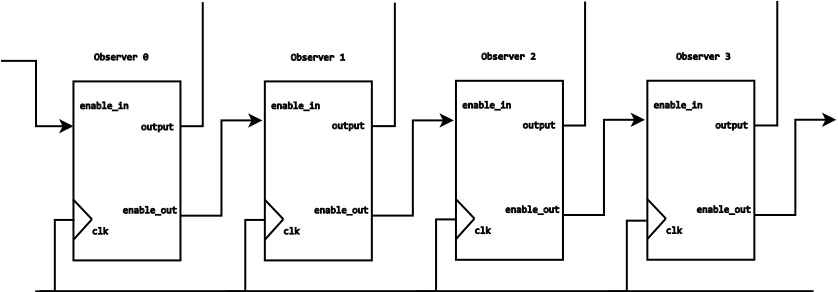
\includegraphics[width=450px]{Chapter2/Figs/Raster/Observer-stage.png}
\caption[Invariant Observer stages in cascade , m=4]{Example for m=4 Invariant Observer Stages concatenated in cascade. }
\label{fig:observerstages}
\end{figure}
\end{center}
This ensures,that these observers are starting delayed,in the meaning of time.\\
Signal \textbf{inc\_tau}(VDHL-Code~\ref{appendix:source:2},line 21) increments the input signal \textbf{invariance\_tau},which represents $\tau+1$ at every execution time.
The asynchronous part works immediately after every change of the system state.(VDHL-Code~\ref{appendix:source:2},line 25 and line 51)
In the following descriptions of the asynchronous parts,only temporary signals are changed,
but these signals transfer their values inside the synchronous part at every clock cycle,except \textbf{inc\_tau} and \textbf{enable\_logic}.
Every of these signals are indicated with "\_next" at the end of their names,but in the following descriptions only their register counterparts will be mentioned. 
\newline \newline
The process entity \textbf{comb\_cycle}(VDHL-Code~\ref{appendix:source:2},line 25) is the description of an internal clock counter which only counts up and down between values 0 and m.
The signal \textbf{cycle} is significant for checking the condition ``(clock mod m) = 0'' from Algorithm~\ref{alg:observerstage}.\\ \\
The process entity \textbf{comb\_logic} implements the real part of the algorithm.
Signal \textbf{count\_p} will be incremented in each clock cycle until it reaches $\tau+1$.
The counter should be initialised to zero (as indicated in the algorithm),but is incremented immediately at every clock cycle.(VDHL-Code~\ref{appendix:source:2},line 55)
Or in other words,if \textbf{count\_p} is reset to zero in a clock cycle,it will be incremented immediately in the "same" clock cycle. 
To demonstrate this fact we have an additional signal \textbf{count}, initialised with 1. 
But this signal is only for reasoning and will be reduced by a syntheses tool.  
The synchronous design is cumbersome in a way,which is due to the way of how the states change.
If the counter is supposed to be incremented after evaluating some conditions,this does not imply an immediate change of the counter.
To overcome this handicap the counter  \textbf{count\_p} is initialised to 2(VDHL-Code~\ref{appendix:source:2},line 56) which means,that 
at every clock cycle we check if the counter count\_p will reach a maximum at the next clock cycle. This enables us to change things on time. 
According to the Algorithm~\ref{alg:observerstage} at line 5,\textbf{count\_p} will only be reset if signal $W(\phi)$ has been evaluated as being not active in \textbf{comb\_cycle}. 
(VDHL-Code~\ref{appendix:source:2},line 56) \\\\
The first if-branch at line 53 of the VDHL-Code~\ref{appendix:source:2} checks two cases.
At first it will be checked if the clock passed m cycles or not and second if the signal \textbf{enable\_logic} is supposed to be active.
The first question is in term of Algorithm~\ref{alg:observerstage},line 2.
The second question concerns the signal \textbf{enable\_logic}. This signal combines \textbf{enable\_in} and \textbf{reset} in one signal. 
If signal \textbf{enable\_logic} is active,means that the observer stage is active and no reset condition happens.
The else-branch of the first if-branch at line 67  of the VDHL-Code~\ref{appendix:source:2} checks the condition in terms of  Algorithm~\ref{alg:observerstage},line 11.
The content of the if-branch (line 53) and the else-branch (67) are nearly the same,but there are two exceptions.
Inside the if-branch,beginning at line 54,the status of signal W($\phi$) will be checked,according to Algorithm~\ref{alg:observerstage},line 3.
And inside the else-branch at line 75,if m cycles are no yet passed and signal \textbf{count\_p} is already  at the maximum,
then signals \textbf{count\_p},\textbf{count} and \textbf{output} keep their old values.
The other parts of \textbf{comb\_cycle} are straightforward,if you compare it with the algorithm.In case the counter \textbf{count\_p} reaches the maximum,
the  \textbf{output} of the observer stage is activated. \\\\
Some points about the improvements made in that design,but it can also be seen as guidelines for further design cases.
It is very important that no Latches are built by the syntheses tool,so every if-branch must contain the same changes on the same signals.
A further point is to reduce the number of if-branches to a minimum. If-branches inside of an If branch extends signal paths and reduce the maximum clock design of the whole design.
In the next chapter we get an overview of the hardware realisation of the current design,which shows us a more visual view on that.
